\chapter{Additional Evaluation Data}
\label{cha:additional_evaluation_data}

\begin{table}[htpb]
    \setlength{\tabcolsep}{0.2em}
    \tiny
    \centering
    \begin{tabular}{l|rrrrrrrrrrrrrrrrrrrrrrrrrrrr}
        \toprule
                & 01 & 02 & 03 & 04 & 05 & 06 & 07 & 08 & 09 & 10 & 11 & 12 & 13 & 14 & 15 & 16 & 17 & 18 & 19 & 20 & 21 & 22 & 23 & 24 & 25 & 26 & 27 & 28 \\
        \midrule
        K6\_S02 & \y & \y & \y & \y & \y & \y & \y & \y & \y & \y & \y & \y & \x & \y & \y & \y & \y & \y & \y & \y & \y & \y & \y & \y & \y & \y & \x & \y \\
        K6\_S03 & \y & \y & \y & \y & \y & \y & \y & \x & \y & \y & \y & \y & \x & \y & \y & \y & \y & \y & \y & \y & \y & \y & \y & \y & \y & \y & \y & \y \\
        K6\_S05 & \y & \y & \y & \y & \y & \y & \y & \y & \y & \y & \y & \y & \y & \y & \y & \y & \y & \y & \y & \x & \y & \y & \x & \x & \x & \y & \y & \y \\
        K6\_S10 & \y & \y & \y & \y & \y & \y & \y & \y & \y & \y & \y & \y & \x & \x & \y & \y & \y & \y & \y & \y & \y & \y & \y & \y & \y & \y & \y & \y \\
        K6\_S11 & \x & \y & \y & \y & \y & \y & \y & \y & \y & \y & \y & \y & \y & \y & \y & \y & \y & \y & \y & \y & \y & \y & \y & \y & \y & \y & \y & \y \\
        K6\_S13 & \y & \y & \y & \y & \y & \y & \y & \y & \y & \y & \y & \y & \y & \y & \y & \y & \y & \y & \y & \y & \y & \y & \y & \y & \y & \y & \y & \y \\
        K6\_S15 & \y & \y & \y & \y & \y & \y & \y & \y & \y & \y & \y & \y & \y & \y & \y & \y & \y & \y & \y & \y & \y & \y & \y & \y & \y & \y & \y & \y \\
        K6\_S16 & \y & \y & \y & \y & \y & \y & \y & \y & \y & \y & \y & \y & \y & \y & \y & \y & \y & \y & \y & \y & \y & \y & \y & \y & \y & \y & \y & \y \\
        K6\_S18 & \y & \y & \y & \y & \y & \y & \y & \y & \y & \y & \y & \y & \y & \y & \y & \y & \y & \y & \y & \y & \y & \y & \y & \y & \y & \y & \y & \y \\
        K6\_S19 & \y & \y & \y & \y & \y & \y & \y & \y & \y & \y & \y & \y & \y & \y & \y & \y & \y & \y & \y & \y & \y & \y & \x & \y & \y & \y & \x & \y \\
        K6\_S27 & \y & \y & \y & \y & \y & \y & \y & \y & \y & \y & \y & \y & \y & \y & \y & \y & \y & \y & \y & \y & \y & \y & \y & \y & \y & \y & \y & \y \\
        K6\_S29 & \y & \y & \y & \y & \y & \y & \y & \y & \y & \y & \y & \y & \y & \y & \y & \y & \y & \y & \y & \y & \y & \y & \y & \y & \y & \y & \y & \y \\
        K6\_S30 & \y & \y & \y & \y & \y & \y & \y & \y & \y & \y & \y & \y & \y & \y & \y & \y & \y & \y & \y & \y & \y & \y & \y & \y & \y & \y & \y & \y \\
        K6\_S31 & \y & \y & \y & \y & \y & \y & \y & \y & \y & \y & \y & \y & \y & \y & \y & \y & \y & \y & \y & \y & \y & \y & \y & \y & \y & \y & \y & \y \\
        K6\_S33 & \y & \y & \y & \y & \y & \y & \y & \x & \y & \y & \y & \y & \y & \y & \y & \y & \y & \y & \y & \y & \y & \y & \y & \y & \y & \y & \y & \y \\
        K7\_S02 & \y & \y & \y & \y & \y & \y & \y & \y & \y & \y & \y & \y & \y & \y & \y & \y & \y & \y & \y & \y & \x & \y & \y & \y & \y & \y & \x & \y \\
        K7\_S03 & \y & \y & \y & \y & \y & \y & \y & \y & \y & \y & \y & \y & \x & \y & \y & \y & \y & \y & \y & \y & \y & \y & \y & \y & \y & \y & \y & \y \\
        K7\_S04 & \y & \y & \y & \y & \y & \y & \y & \y & \y & \y & \y & \y & \y & \y & \y & \y & \y & \y & \y & \y & \y & \y & \y & \y & \y & \y & \y & \y \\
        K7\_S05 & \y & \y & \y & \y & \y & \y & \y & \y & \y & \y & \y & \y & \y & \y & \y & \y & \y & \y & \y & \y & \y & \y & \y & \y & \y & \y & \y & \y \\
        K7\_S06 & \y & \y & \y & \y & \y & \y & \y & \y & \y & \y & \y & \y & \y & \y & \y & \y & \y & \y & \y & \y & \y & \y & \y & \y & \y & \y & \y & \y \\
        K7\_S08 & \y & \y & \y & \y & \y & \y & \y & \y & \y & \y & \y & \y & \y & \y & \y & \y & \y & \y & \y & \y & \y & \y & \y & \y & \y & \y & \y & \y \\
        K7\_S10 & \y & \y & \y & \y & \y & \y & \y & \y & \y & \y & \y & \y & \y & \y & \y & \y & \y & \y & \y & \y & \x & \y & \y & \y & \y & \y & \y & \y \\
        K7\_S11 & \y & \y & \y & \y & \y & \y & \y & \y & \y & \y & \y & \y & \y & \y & \y & \y & \y & \y & \y & \y & \y & \y & \y & \y & \y & \y & \y & \y \\
        K7\_S12 & \y & \y & \y & \y & \y & \y & \y & \y & \y & \y & \y & \y & \y & \x & \y & \y & \y & \y & \y & \y & \y & \y & \y & \y & \y & \y & \y & \y \\
        K7\_S14 & \y & \y & \y & \y & \y & \y & \y & \y & \y & \y & \y & \y & \y & \y & \y & \y & \y & \y & \y & \y & \y & \y & \y & \y & \y & \y & \y & \y \\
        K7\_S15 & \y & \y & \y & \y & \y & \y & \y & \y & \y & \y & \y & \y & \y & \y & \y & \y & \y & \y & \y & \y & \y & \y & \y & \y & \y & \y & \y & \y \\
        K7\_S16 & \y & \y & \y & \x & \y & \y & \y & \y & \y & \y & \y & \y & \y & \y & \y & \y & \y & \y & \y & \y & \y & \y & \y & \y & \y & \y & \y & \y \\
        K7\_S17 & \y & \y & \y & \y & \y & \y & \y & \y & \y & \y & \y & \y & \y & \y & \y & \y & \y & \y & \x & \y & \x & \y & \x & \x & \y & \y & \y & \y \\
        K7\_S19 & \y & \y & \y & \y & \y & \y & \y & \y & \y & \y & \y & \y & \y & \y & \y & \y & \y & \y & \y & \y & \y & \y & \y & \y & \y & \y & \y & \y \\
        K7\_S20 & \y & \y & \y & \y & \y & \y & \y & \y & \y & \y & \y & \y & \y & \y & \y & \y & \y & \y & \y & \y & \y & \y & \y & \y & \y & \y & \y & \y \\
        K7\_S26 & \y & \y & \y & \y & \y & \y & \y & \y & \y & \y & \y & \y & \y & \y & \y & \y & \y & \y & \y & \y & \y & \y & \y & \y & \y & \y & \y & \y \\
        \bottomrule
    \end{tabular}
    \caption{Inconsistency matrix for test suite T1 (normal tests)}
    \label{tab:inconsistencies_matrix_normal}
    \setlength{\tabcolsep}{\defaulttabcolsep}
\end{table}

\begin{table}[htpb]
    \setlength{\tabcolsep}{0.2em}
    \tiny
    \centering
    \begin{tabular}{l|rrrrrrrrrrrrrrrrrrrr}
        \toprule
               & 01 & 02 & 03 & 04 & 05 & 06 & 07 & 08 & 09 & 10 & 11 & 12 & 13 & 14 & 15 & 16 & 17 & 18 & 19 & 20 \\
        \midrule
        K6\_S02 & \y & \y & \y & \y & \y & \y & \y & \y & \y & \y & \y & \y & \y & \y & \y & \x & \x & \y & \y & \y \\
        K6\_S03 & \y & \y & \y & \y & \y & \y & \y & \y & \y & \y & \y & \y & \y & \y & \x & \y & \y & \y & \y & \y \\
        K6\_S05 & \y & \y & \y & \y & \y & \y & \y & \y & \y & \y & \y & \x & \y & \y & \y & \y & \y & \y & \y & \y \\
        K6\_S10 & \y & \y & \y & \y & \y & \y & \y & \y & \y & \y & \y & \y & \y & \y & \y & \x & \y & \y & \x & \x \\
        K6\_S11 & \y & \y & \y & \y & \y & \y & \y & \y & \y & \y & \y & \y & \y & \y & \y & \y & \y & \y & \y & \y \\
        K6\_S13 & \y & \y & \y & \y & \y & \y & \y & \y & \y & \y & \y & \y & \y & \y & \y & \y & \y & \y & \y & \y \\
        K6\_S15 & \y & \y & \y & \y & \y & \y & \y & \y & \y & \y & \y & \y & \y & \y & \y & \y & \y & \y & \y & \y \\
        K6\_S16 & \y & \y & \y & \y & \y & \y & \y & \y & \y & \y & \y & \y & \y & \y & \y & \y & \y & \y & \y & \y \\
        K6\_S18 & \y & \y & \y & \y & \y & \y & \y & \y & \y & \y & \y & \y & \y & \y & \y & \y & \y & \y & \y & \y \\
        K6\_S19 & \y & \y & \y & \y & \y & \y & \y & \y & \y & \y & \y & \y & \y & \y & \y & \y & \y & \y & \x & \y \\
        K6\_S27 & \y & \y & \y & \y & \y & \y & \y & \y & \y & \y & \y & \y & \y & \y & \y & \y & \y & \y & \y & \y \\
        K6\_S29 & \y & \y & \y & \y & \y & \y & \y & \y & \y & \y & \y & \y & \y & \y & \y & \y & \y & \y & \y & \y \\
        K6\_S30 & \y & \y & \y & \y & \y & \y & \y & \y & \y & \y & \y & \y & \x & \x & \y & \y & \y & \y & \y & \y \\
        K6\_S31 & \y & \y & \y & \y & \y & \y & \y & \y & \y & \y & \y & \y & \y & \y & \y & \y & \y & \y & \y & \y \\
        K6\_S33 & \y & \y & \y & \y & \y & \y & \y & \y & \y & \y & \y & \x & \y & \y & \x & \y & \y & \y & \y & \y \\
        K7\_S02 & \y & \y & \y & \y & \y & \y & \y & \y & \y & \y & \y & \y & \y & \y & \y & \y & \y & \y & \y & \y \\
        K7\_S03 & \y & \y & \y & \y & \y & \y & \y & \y & \y & \y & \y & \y & \y & \y & \y & \y & \y & \y & \y & \y \\
        K7\_S04 & \y & \y & \y & \y & \y & \y & \y & \y & \y & \y & \y & \y & \y & \y & \y & \y & \y & \y & \y & \y \\
        K7\_S05 & \y & \y & \y & \y & \y & \y & \y & \y & \y & \y & \y & \y & \y & \y & \y & \y & \y & \y & \y & \y \\
        K7\_S06 & \y & \y & \y & \y & \y & \y & \y & \y & \y & \y & \y & \y & \y & \y & \y & \y & \y & \y & \y & \y \\
        K7\_S08 & \y & \y & \y & \y & \y & \y & \y & \y & \y & \y & \y & \x & \y & \y & \y & \y & \y & \y & \y & \y \\
        K7\_S10 & \y & \y & \y & \y & \y & \y & \y & \y & \y & \y & \y & \y & \y & \y & \y & \y & \y & \y & \y & \y \\
        K7\_S11 & \y & \y & \y & \y & \y & \y & \y & \y & \y & \y & \y & \y & \y & \y & \y & \y & \y & \y & \y & \y \\
        K7\_S12 & \y & \y & \y & \y & \y & \y & \y & \y & \y & \y & \y & \y & \y & \y & \y & \y & \y & \y & \y & \y \\
        K7\_S14 & \y & \y & \y & \y & \y & \y & \y & \y & \y & \y & \y & \y & \y & \y & \y & \y & \y & \y & \y & \y \\
        K7\_S15 & \y & \y & \y & \y & \y & \y & \y & \y & \y & \y & \y & \y & \y & \y & \y & \y & \y & \y & \y & \y \\
        K7\_S16 & \y & \x & \y & \y & \y & \y & \y & \y & \y & \y & \y & \y & \y & \y & \y & \y & \y & \y & \y & \y \\
        K7\_S17 & \y & \y & \y & \y & \x & \y & \y & \y & \y & \y & \y & \y & \y & \y & \y & \y & \x & \y & \y & \y \\
        K7\_S19 & \y & \y & \y & \y & \y & \y & \y & \y & \y & \y & \y & \y & \y & \y & \y & \y & \y & \y & \y & \y \\
        K7\_S20 & \y & \y & \y & \y & \y & \y & \y & \y & \y & \y & \y & \y & \y & \y & \x & \y & \y & \y & \y & \y \\
        K7\_S26 & \y & \y & \y & \y & \y & \y & \y & \y & \y & \y & \y & \y & \y & \y & \y & \y & \y & \y & \y & \y \\
        \bottomrule
    \end{tabular}
    \caption{Inconsistency matrix for test suite T2 (input-independent / constraint-only tests)}
    \label{tab:inconsistencies_matrix_constraint}
    \setlength{\tabcolsep}{\defaulttabcolsep}
\end{table}

\begin{table}[htpb]
    \setlength{\tabcolsep}{0.2em}
    \tiny
    \centering
    \begin{tabular}{l|rrrrrrrrrrrrrrrrrr}
        \toprule
                & 01 & 02 & 03 & 04 & 05 & 06 & 07 & 08 & 09 & 10 & 11 & 12 & 13 & 14 & 15 & 16 & 17 & 18 \\
        \midrule
        K6\_S02 & \y & \y & \y & \y & \y & \y & \y & \y & \y & \y & \y & \y & \y & \x & \y & \y & \x & \y \\
        K6\_S03 & \y & \y & \y & \y & \y & \y & \y & \y & \y & \y & \y & \x & \y & \y & \y & \y & \y & \y \\
        K6\_S05 & \y & \y & \y & \y & \y & \y & \y & \y & \y & \y & \y & \x & \x & \x & \x & \y & \y & \y \\
        K6\_S10 & \y & \x & \x & \y & \y & \y & \y & \y & \y & \y & \y & \y & \x & \x & \y & \x & \y & \y \\
        K6\_S11 & \y & \y & \y & \y & \y & \y & \y & \y & \y & \y & \y & \x & \y & \y & \y & \y & \y & \y \\
        K6\_S13 & \y & \y & \y & \y & \y & \y & \y & \y & \y & \y & \y & \y & \y & \y & \y & \y & \y & \y \\
        K6\_S15 & \y & \y & \y & \y & \y & \y & \y & \y & \y & \y & \y & \y & \y & \y & \y & \y & \y & \y \\
        K6\_S16 & \y & \y & \y & \y & \y & \y & \y & \y & \y & \y & \y & \y & \y & \y & \y & \y & \y & \y \\
        K6\_S18 & \y & \x & \x & \y & \y & \y & \y & \y & \y & \y & \y & \y & \x & \y & \y & \y & \y & \y \\
        K6\_S19 & \y & \y & \y & \y & \y & \y & \y & \y & \y & \y & \y & \y & \y & \y & \x & \y & \y & \y \\
        K6\_S27 & \y & \y & \y & \y & \y & \y & \y & \y & \y & \y & \y & \y & \y & \y & \y & \y & \y & \y \\
        K6\_S29 & \y & \y & \x & \y & \y & \y & \y & \y & \y & \y & \y & \y & \y & \y & \x & \y & \x & \y \\
        K6\_S30 & \y & \x & \x & \y & \y & \y & \y & \y & \y & \y & \y & \y & \x & \x & \y & \y & \y & \y \\
        K6\_S31 & \y & \y & \y & \y & \y & \y & \y & \x & \y & \y & \y & \y & \y & \y & \y & \y & \y & \y \\
        K6\_S33 & \y & \y & \y & \y & \y & \y & \y & \x & \y & \y & \y & \x & \y & \y & \y & \y & \y & \y \\
        K7\_S02 & \y & \x & \y & \y & \y & \y & \y & \y & \y & \y & \y & \y & \y & \y & \y & \y & \y & \y \\
        K7\_S03 & \y & \x & \x & \y & \y & \y & \y & \x & \y & \y & \y & \x & \y & \y & \y & \y & \y & \y \\
        K7\_S04 & \y & \x & \x & \y & \y & \y & \y & \y & \y & \y & \y & \y & \y & \y & \x & \x & \y & \y \\
        K7\_S05 & \y & \y & \y & \y & \y & \y & \y & \y & \y & \y & \y & \y & \y & \y & \y & \x & \y & \y \\
        K7\_S06 & \y & \y & \y & \y & \y & \y & \y & \y & \y & \y & \y & \y & \y & \y & \y & \y & \y & \y \\
        K7\_S08 & \y & \x & \x & \y & \y & \y & \y & \y & \y & \y & \y & \y & \y & \y & \y & \y & \y & \y \\
        K7\_S10 & \y & \x & \x & \y & \y & \y & \y & \y & \y & \y & \y & \x & \y & \y & \x & \y & \y & \y \\
        K7\_S11 & \y & \y & \y & \y & \y & \y & \y & \y & \y & \y & \y & \y & \y & \y & \y & \y & \y & \y \\
        K7\_S12 & \y & \y & \y & \y & \y & \y & \y & \y & \y & \y & \y & \y & \x & \x & \x & \x & \y & \y \\
        K7\_S14 & \y & \y & \x & \y & \y & \y & \y & \y & \y & \y & \y & \y & \x & \x & \y & \x & \y & \y \\
        K7\_S15 & \y & \y & \y & \y & \y & \y & \y & \x & \y & \y & \y & \x & \y & \y & \y & \y & \y & \y \\
        K7\_S16 & \y & \x & \y & \y & \y & \y & \y & \y & \y & \y & \y & \x & \y & \y & \x & \y & \y & \y \\
        K7\_S17 & \y & \y & \y & \y & \x & \y & \y & \y & \y & \y & \y & \x & \y & \y & \x & \y & \y & \y \\
        K7\_S19 & \y & \y & \y & \y & \y & \y & \y & \x & \y & \y & \y & \y & \x & \y & \y & \y & \y & \y \\
        K7\_S20 & \y & \x & \x & \y & \y & \y & \y & \y & \y & \y & \y & \y & \y & \y & \y & \y & \y & \y \\
        K7\_S26 & \y & \y & \y & \y & \y & \y & \y & \y & \y & \y & \y & \y & \y & \x & \x & \x & \x & \y \\
        \bottomrule
    \end{tabular}
    \caption{Inconsistency matrix for test suite T3 (random input tests)}
    \label{tab:inconsistencies_matrix_random}
    \setlength{\tabcolsep}{\defaulttabcolsep}
\end{table}

\begin{figure}[htpb]
    \centering
    \fbox{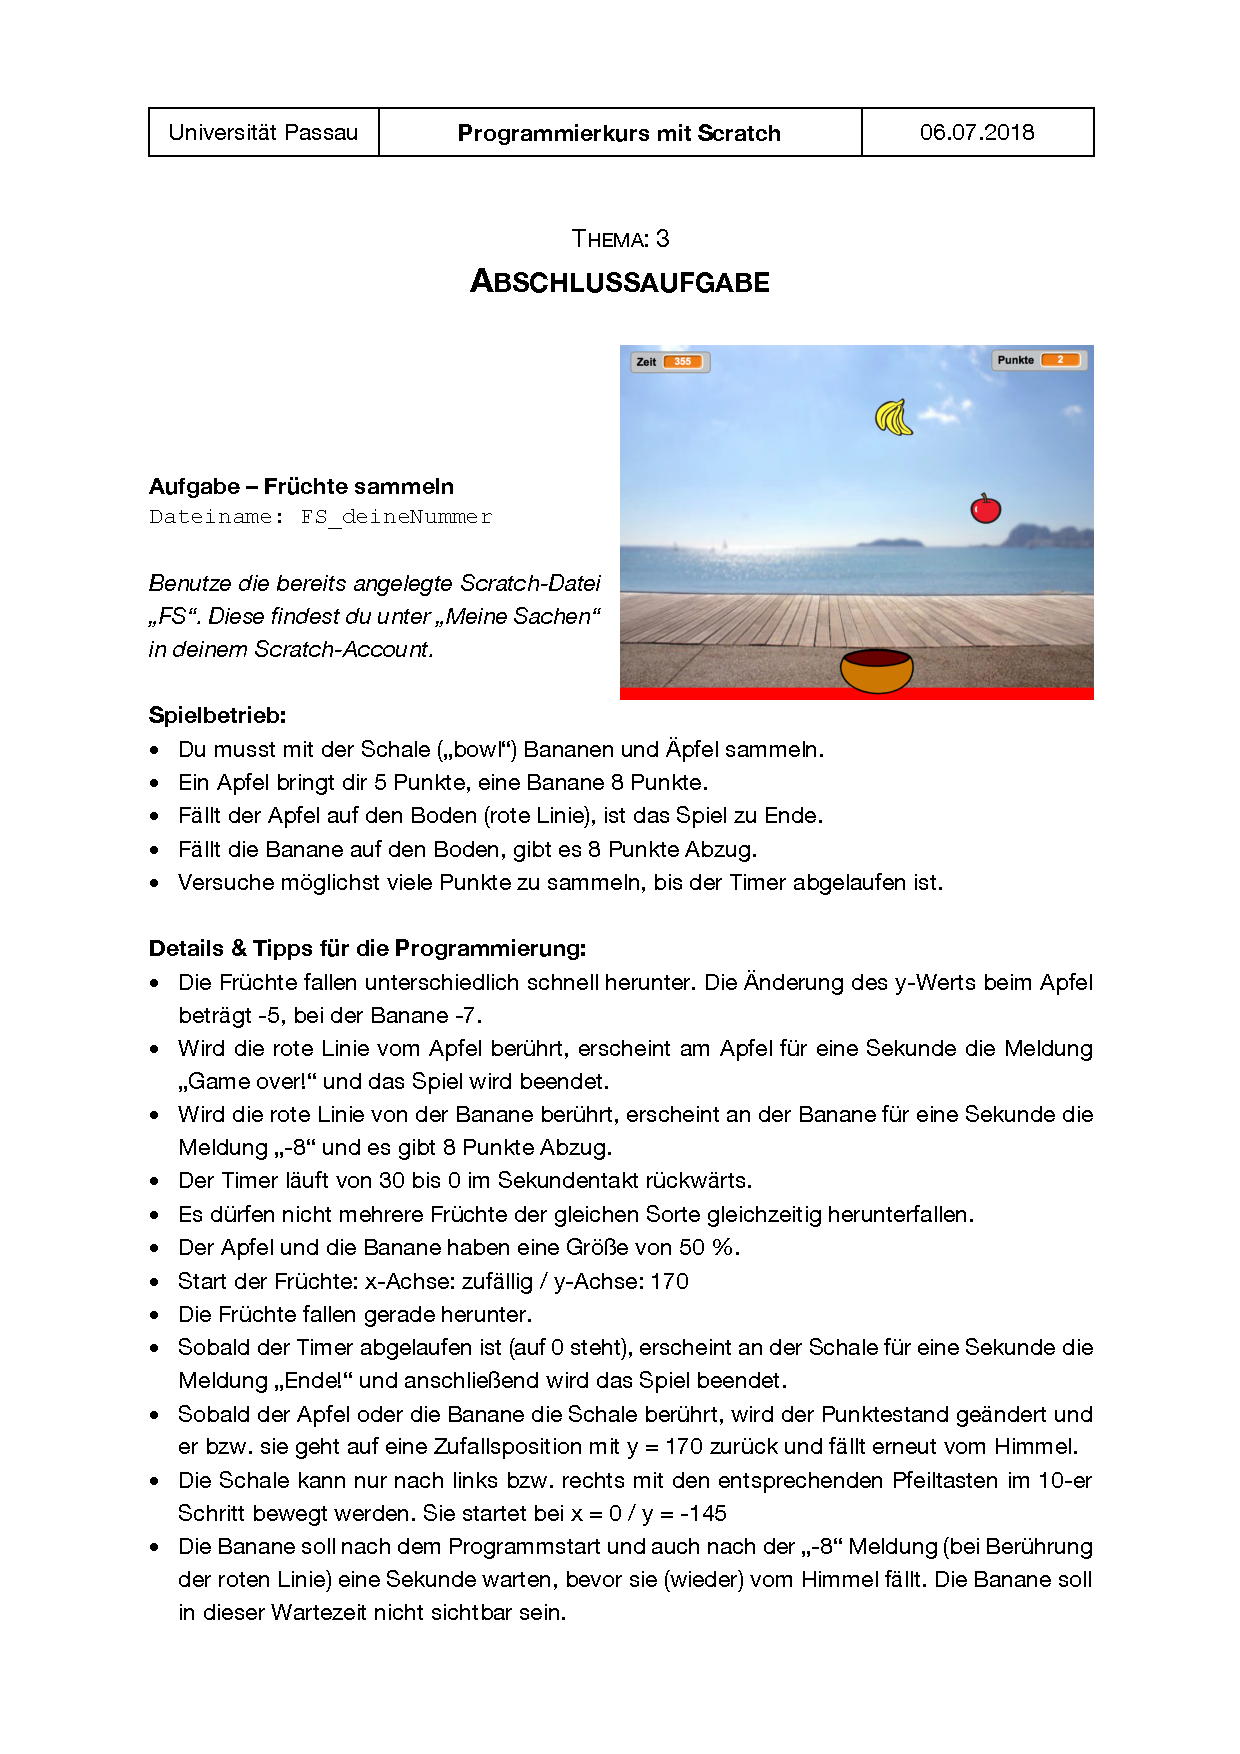
\includegraphics[width=\textwidth]{task-description}}
    \caption{Task description for the catching game (by Sebastian Keller \cite{keller})}
    \label{fig:catching_game_task_description}
\end{figure}

\begin{listing}[htpb]
    \centering

    \begin{subfigure}[b]{.40\textwidth}
        \begin{minted}[autogobble, breaklines, linenos, fontsize=\tiny, framesep=2mm, frame=lines]{javascript}
            const names = [
                'callbacks-before',
                'random-inputs',
                'inputs',
                'sprites',
                'scratch',
                'callbacks-after',
                'constraints'
            ];

            let currentTimestamp;
            let currentRecord;
            let records;

            const resetRecords = function () {
                records = [];
            };

            const startRecord = function () {
                currentTimestamp = window.performance.now();
                currentRecord = [];
            };

            const record = function () {
                currentRecord.push(window.performance.now() - currentTimestamp);
            };

            const endRecord = function () {
                records.push(currentRecord);
            };

            const getRecords = function () {
                return {
                    names,
                    records
                };
            };
        \end{minted}
        \vspace{-\bigskipamount}
        \caption{Helper methods}
    \end{subfigure}
    \hspace{.08\textwidth}
    \begin{subfigure}[b]{.40\textwidth}
        \begin{minted}[autogobble, breaklines, linenos, fontsize=\tiny, framesep=2mm, frame=lines]{javascript}
            step () {
                startRecord();

                this.callbacks.callCallbacks(false);
                record();

                if (!this.running) {
                    endRecord();
                    return;
                }

                this.randomInputs.performRandomInput();
                record();

                this.inputs.performInputs();
                record();

                this.sprites.update();
                record();

                this.vm.runtime._step();
                record();

                if (!this.running) {
                    endRecord();
                    return;
                }

                this.callbacks.callCallbacks(true);
                record();

                if (!this.running) {
                    endRecord();
                    return;
                }

                const rv = this.constraints.checkConstraints();
                record();

                endRecord();

                return rv;
            }
        \end{minted}
        \vspace{-\bigskipamount}
        \caption{Modified step procedure}
    \end{subfigure}
    \caption{Modified Whisker step procedure for execution time measurement}
    \label{lst:time_measurement_code}
\end{listing}
